\documentclass[a4paper,10pt]{article}
\usepackage[utf8]{inputenc}
\usepackage{amsmath}
\usepackage{graphicx}
\usepackage{hyperref}

%opening
\title{WP 1.1 Mathematical Foundations}
\author{J. G. P. Vermeulen}

\begin{document}

\maketitle

\section{Contents}

This works package details the mathematical foundations for the thesis work. This will be split up into several sections:
\begin{itemize}
\item Coordinate systems and transformations
\item Three-body orbital mechanics (summary)
\item Definitions for the numerical methods
\item Definitions for the Kalman filter methods
\item Definitions for the neural networks
\end{itemize}

\section{Coordinate systems and transformations}
This section will detail the necessary coordinate systems and corresponding transformations.\\

Often, an orbit is expressed in terms of the Keplerian orbital elements:
\begin{itemize}
\item Eccentricity $e$
\item Semi-major axis $a$
\item Inclination $i$
\item Right Ascension of the Ascending Node $\Omega$
\item Argument of Periapsis $\omega$
\item True anomaly at Epoch $\theta$
\end{itemize}

These elements provide a full specification of the orbit in 3D, but they are not that useful for our application. Therefore, some additional coordinate frames are defined, along with transformations. The most important frames are the heliocentric and the geocentric reference frames. Additionally, the camera reference frame of the spacecraft needs to be specified.

\subsection{Heliocentric reference frame}
The heliocentric, or \textit{non-rotating heliocentric ecliptic} reference frame is a non-rotating, quasi-inertial reference frame. As XY-plane, the plane of the ecliptic is used. Therefore, the Z+ direction is perpendicular to the plane of the ecliptic, pointing North. The X+ direction points towards the vernal equinox (first point of Aries). The Y+ direction completes the right-handed coordinate system. The coordinate system is centered on the center of mass of the Sun.

\subsection{Geocentric reference frame}
The geocentric reference frame that will be used is the \textit{non-rotating geocentric ecliptic} reference frame. The geocentric reference frame is defined similar to the heliocentric frame, but centered on the center of mass of the Earth. Note that all axes are parallel: celestial north and the first point of Aries are located at an infinite distance from the origin, and therefore the directions from the Sun and from Earth are parallel.

\subsection{Spacecraft camera reference frame}
To specify the observations of the target in the spacecraft's camera, the spacecraft camera reference frame is defined. In order to specify this coordinate frame, first the spacecraft (quasi-)inertial reference frame is defined. The spacecraft inertial frame is defined similar to the heliocentric and geocentric reference frames, but with the coordinate system centered on the spacecraft center of mass. From this, a simplifying assumption is made: it is assumed the spacecraft focal plane and optical axis coincide with its center of mass. As the dimensions of the spacecraft are negligible compared to the distance to the targets, this assumption is justified. From here, the spacecraft camera reference frame can be defined as the reference frame centered on the intersection of the optical axis of the camera and the camera focal plane, with axis L+ pointing in the direction of the optical axis of the camera (``out'' from the focal plane), M+ pointing to the left and N+ completing the right-handed system by pointing up, both as seen from the focal plane. This is seen in \autoref{fig:cameracoordinates}.

\begin{figure}[htbp]
 \centering
 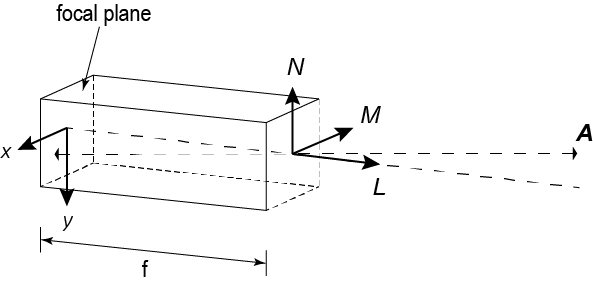
\includegraphics[width=0.6\textwidth]{cameracoordinates.png}
 \caption{Camera reference frame}
 \label{fig:cameracoordinates}
\end{figure}

TRANSFORMATIONS

\section{Alternative coordinate systems}
A problem that will be encountered later in the process is the ``conversion'' from a preliminary orbit determination to an impact threat assessment. For this, it might be necessary to tell the system where Earth is. (alternatively, other metrics such as MOID could be looked at, leading to a system where the target is analysed in more detail from Earth). Instead of giving the system a measure of Earth's location, it might be convenient to define a coordinate system in which both Earth and the Sun (as it is the main gravitational attractor) are fixed. We shall define the Sun-Earth ecliptic reference frame as the right-handed frame with the origin at the center of the Sun, the Z+ axis pointing North perpendicular to the ecliptic, the X+ axis pointing through the center of Earth, and the Y+ axis completing the right-handed system. \\

The advantage of this system is obvious: if we assume Earth's orbit to be circular, the position of Earth will always be $[1, 0, 0]^T~AU$, and therefore the problem simplifies to determining the hazard to that point. However, as the reference frame is no longer non-rotating, the dynamics of the motion vastly complicate.

\section{Transformations}

Most coordinate transformations that are required are quite straightfoward. The transformation between heliocentric frame $h$, geocentric frame $e$ and spacecraft centered frame $s$ can be performed through vector addition. Example for vector $\vec{r}$:
\begin{equation}
 \vec{r}^s = \vec{r}^h - \vec{r_s}^h
\end{equation}
With $\vec{r_s}^h$ denoting the position of the spacecraft in the heliocentric frame. In words: the position of the target in the spacecraft-centered frame is the difference of the position of the target and the position of the spacecraft in any of the other reference frames. \\

Thus, when the position of Sun, Earth and spacecraft are known in each of the respective frames, the coordinate transformation is straightforward. The other coordinate frames require a more elaborate transformation to achieve. The Sun-Earth ecliptic frame $r$ (for rotating) can be achieved by a rotation of the heliocentric frame around the Z-axis. If we define the true anomaly of the Earth $\theta_e$ as 0 at the vernal equinox, we find that:

\begin{equation}
 \vec{r}^r = \mathbf{R_3}(\theta_e) \vec{r}^h
\end{equation}

With $\mathbf{R_3}$ denoting a rotation around the third axis. Similarly, the camera coordinate frame can be achieved by a rotation matrix $\mathbf{C}$ which can be given in terms of twist angle $\phi$, right ascension $\alpha$ and declination $\delta$:
\begin{equation}
 \mathbf{C} = \mathbf{R_3}(\phi)\mathbf{R_1}(90^\circ - \delta)\mathbf{R_3}(\alpha + 90^\circ)
\end{equation}
or:
\begin{equation}
 \mathbf{R_3}(\phi + 90^\circ)\mathbf{R_2}(90^\circ - \delta)\mathbf{R_3}(\alpha)
\end{equation}
Then:
\begin{equation}
 \vec{r}^c = \mathbf{C}(\alpha, \delta, \phi)\vec{r}^s
\end{equation}
The rotation matrices are given by:
\begin{align}
 \mathbf{R_1}(\theta) &= \begin{bmatrix}1 & 0 & 0 \\ 0 & \cos \theta & -\sin \theta \\ 0 & \sin \theta & \cos \theta \end{bmatrix} \\
 \mathbf{R_2}(\theta) &= \begin{bmatrix} \cos \theta & 0 & - \sin \theta \\ 0 & 1 & 0 \\ - \sin \theta & 0 & \cos \theta \end{bmatrix} \\
 \mathbf{R_3}(\theta) &= \begin{bmatrix} \cos \theta & -\sin \theta & 0 \\ \sin \theta & \cos \theta & 0 \\ 0 & 0 & 1 \end{bmatrix}
\end{align}







\section{Two- and Three-body Orbital Mechanics}

The equations of motion need to be known in order to accurately model the asteroids and to e.g. apply the kalman filter and parts of the numerical methods. The motion of the spacecraft around the Sun is governed soleley by gravity. By assuming the Sun to be at rest (a fair assumption, as $m_{S/C} << m_\odot$), only gravitational force is to be considered:

\begin{equation}
 \frac{d^2 \vec{r}}{dt^2} = \frac{\mu_\odot}{||r||^3}\vec{r}
\end{equation}

Consequently, velocity and position are obtained by integration of the acceleration. Or, in equations, the position of the spacecraft at time $t=T$ can be determined from its position and velocity at time $t=0$:
\begin{align}
\vec{r}(t=T) &= \vec{r}(t=0) + \int_0^T \frac{d \vec{r}}{dt} dt \\
\frac{d \vec{r}}{dt}(t=T) &= \frac{d \vec{r}}{dt}(t=0) + \int_0^T \frac{d^2 \vec{r}}{dt^2} dt \\
\frac{d^2 \vec{r}}{dt^2}(t=T) &= \frac{\mu_\odot}{||r(t=T)||^3}\vec{r}(t=T)
\end{align}

If a discrete-time solution is required, the following result is obtained (with velocity $v$ and acceleration $a$:
\begin{align}
 \vec{r}(T+\Delta t) &= \vec{r}(T) + \vec{v}(T)\Delta t \\
 \vec{v}(T+\Delta t) &= \vec{v}(T) + \vec{a}(T)\Delta t \\
 \vec{a}(T+\Delta t) &= \frac{\mu_\odot}{||r(T+\Delta t)||^3}\vec{r}(T + \Delta t)
\end{align}
But alternate integration schemes are of course possible (and might be necessary for stability over longer timescales).\\

The resulting trajectory for the two-body problem is simple:

\begin{equation}
 r(\theta) = \frac{a(1-e^2)}{1+e \cos (\theta)}
\end{equation}

As the motion is in a single plane, it is only necessary to know the distance to the barycenter (which can be assumed to coincide with the Sun), and the true anomaly $\theta$. The orbital elements $\Omega$, $i$ and $\omega$ can be seen as Euler angles rotating the coordinate system. If we define the \textit{orbital reference frame} $o$ with X+ towards the periapsis, Z+ perpendicular to the plane of the orbit and Y+ completing the coordinate system right-handed, we can define the following transformations:

\begin{equation}
 \begin{bmatrix}
  x_o \\ y_o \\ z_o
 \end{bmatrix}
 =
 \begin{bmatrix}
  \cos \omega & \sin \omega & 0 \\
  - \sin \omega & \cos \omega & 0 \\
  0 & 0 & 1
 \end{bmatrix}
 \begin{bmatrix}
  1 & 0 & 0 \\
  0 & \cos i & \sin i \\
  0 & -\sin i & \cos i
 \end{bmatrix}
 \begin{bmatrix}
  \cos \Omega & \sin \Omega & 0 \\
  - \sin \Omega & \cos \Omega & 0 \\
  0 & 0 & 1
 \end{bmatrix}
 \begin{bmatrix}
  x_h \\ y_h \\ z_h
 \end{bmatrix}
\end{equation}

Finding the inverse is straightforward: firstly, one should note all matrices are diagonal and thus easily invertible. However, perhaps more intuitively, the rotation sequence can be ``reversed'' by simply reversing the order of the matrices and inverting the sign of the angles (essentially ``rotating'' the system ``back'' into its original orientation):

\begin{equation}
 \begin{bmatrix}
  x_h \\ y_h \\ z_h
 \end{bmatrix}
 =
 \begin{bmatrix}
  \cos -\Omega & \sin -\Omega & 0 \\
  -\sin -\Omega & \cos -\Omega & 0 \\
  0 & 0 & 1
 \end{bmatrix}
 \begin{bmatrix}
  1 & 0 & 0 \\
  0 & \cos -i & \sin -i \\
  0 & -\sin -i & \cos -i
 \end{bmatrix}
 \begin{bmatrix}
  \cos -\omega & \sin -\omega & 0 \\
  - \sin -\omega & \cos -\omega & 0 \\
  0 & 0 & 1
 \end{bmatrix}
 \begin{bmatrix}
  x_o \\ y_o \\ z_o
 \end{bmatrix}
\end{equation}

Lastly, conversion from $r, \theta$ to $x_o, y_o, z_o$ is simple (note that $z_o$ is always zero in the two-body solution as the orbit is planar):
\begin{equation}
 \begin{bmatrix}
  x_o \\ y_o \\ z_o
 \end{bmatrix}
 =
 \begin{bmatrix}
  \cos \theta \\ \sin \theta \\ 0
 \end{bmatrix}
 r
\end{equation}

\section{Relative position and motion}

Although we might assume the Sun remains stationary under the gravitational influence of our spacecraft and the target asteroid, such simplifying assumptions can not be made for the relative motion of the target with respect to the spacecraft: it would be impossible (or at best, comically impractical) to have our spacecraft observing from the Sun. Therefore a solution is needed to obtain the relative positions and motions over time.\\

Firstly, some notation: $r_t^h$ and $r_s^h$ represent the radius vectors of the target and spacecraft in the heliocentric frame (vector symbol omitted for easier reading). The relative position of the target (in other words: the position of the target $t$ in spacecraft reference frame $s$) is then given by:
\begin{equation}
 r_t^s = r_t^h - r_s^h
\end{equation}
Unfortunately, this is where the straightforward solutions end. As the problem becomes dependent on time, we require an expression of the position along the orbit as a function of time, in other words, we are looking for $\theta(t)$. This can be determined through using the \textit{eccentric anomaly} $E$ and the \textit{mean anomaly} $M$:
\begin{align}
 M(t) &= \sqrt{\frac{\mu_\odot}{a^3}}(t-t_0) \\
 E(t) - e \sin E &= M(t) \\
 \theta (t) &= \cos ^{-1} \left(\frac{\cos E(t) - e}{1 - e \cos E(t)}\right)
\end{align}
Unfortunately the expression for $E(t)$ has no closed-form solution. Therefore, a numerical approach is required. (http://www.alpheratz.net/dynamics/twobody/KeplerIterations\_summary.pdf) describe an approach that is both computationally efficient as well as mathematically straightforward. For the derivation, please refer to their paper. Firstly, a start value can be determined through iteration of:
\begin{equation}
 E_k = M + e\sin E_{k-1}
\end{equation}
As $E=M$ in the limit where $e=0$. The authors suggest using a third-order as a good compromise of programming complexity and accuracy:
\begin{equation}
 E_{start} = M + \left( - \frac{e^3}{2} + e + \left(e^2 + \frac{3 e^3 \cos M}{2} \right)\cos M \right)\sin M
\end{equation}



Continuing, they define a function $f(x)$:
\begin{equation}
 f(x) = x - e \sin x - M
\end{equation}
Where $f(x) = 0$ corresponds to $x = E$, the error is defined as $\epsilon \equiv x-E$. Performing a Taylor series expansion about $x=E$ yields:
\begin{equation}
 f(E) = f(x-\epsilon) = x - e \sin x - M - (1 - e \cos x)\epsilon + \frac{1}{2} \epsilon ^2 e \sin x - \frac{1}{6} \epsilon^3 e \cos x + \dots
\end{equation}
The third-order approximation can be solved for $\epsilon$ as:
\begin{equation}
 \epsilon_{n+1} = \frac{x_n - e \sin x_n - M}{1 - e \cos x_n - \frac{1}{2}\left(e \sin x_n - \frac{1}{3} e \cos x_n \cdot \epsilon_n \right)\epsilon_n}
\end{equation}
After which we can iterate by simply:
\begin{equation}
 E_{n+1} = E_n - \epsilon_n
\end{equation}





\section{Numerical Methods}

As mentioned in the literature study, the numerical methods based on the method of very short arcs require knowing the parameter space of the targets. As determined by the original authors, there are some initial requirements:
\begin{itemize}
 \item If the object is within the SoI of Earth, it can't be orbitting Earth.
 \item The object should orbit the sun
 \item The object should have a reasonable magnitude
\end{itemize}
These can be further defined when examining whether an asteroid is dangerous:
\begin{itemize}
 \item The object should be a NEA, i.e. $q \leq 1.017\mathrm{AU}$ and $Q \geq 0.983\mathrm{AU}$
 \item The object should be large enough to cause damage, i.e. $D\geq30\mathrm{m}$, corresponding to $H \leq 25$
 \item The object should be small enough that there's a chance it hasn't been found, i.e. $H \geq 15$
\end{itemize}

This leaves the question of how to efficiently estimate the parameter space. Essentially, we can accomplish this by getting an estimate of $\vec{r}$ and $\dot{\vec{r}}$. Imagine extending an imaginary line from the camera in the direction of the target during a measurement. It is known the target is somewhere along this line. Thus, this constrains the possibilities for $\vec{r}$ to a small subspace. When taking a second measurement, we can fit a straight line to the trajectory (which should be accurate for a short timestep; for higher timesteps the method of short arcs is unneccessary). This allows computation of $\dot{\vec{r}}$. With both of these vectors known, the orbit is essentially determined. If more than 2 measurements are available, the straight line can be fit more accurately using e.g. a least-squares estimation.\\

The process of determining the admissible values of $\vec{r}$ is as follows:
\begin{enumerate}
 \item Use the apparent magnitude of the object to determine the range of $||r||$
 \item Perform coordinate transforms to get $\vec{r}$ in the heliocentric reference frame
 \item Repeat step 1 for the second measurement, using the constraints on orbital energy to determine $\dot{\vec{r}}$
 \item Calculate risk to Earth using monte-carlo methods.
\end{enumerate}

The first step assume phase integral is:
\begin{equation}
 \phi(\alpha) = |\cos{\frac{1}{2}\alpha}| = \sqrt{\frac{1+\cos \alpha}{2}}
 \label{eq:phase}
\end{equation}


With absolute magnitude $H$ and apparent magnitude $m$, we can find for body $B$ orbiting Sun $S$ as seen from observer $O$, $d$ in AU:

\begin{equation}
 H = m - 5 \log _{10} \left(d_{BS}d_{BO}\right) + 2.5\log _{10} \phi(\alpha)
\end{equation}

Initially, I think it's best to just do this iteratively. There will be a large range of initial $\vec{r}$ values. However, the second step will have a much smaller solution space because of the other restrictions. Then, using e.g. scikit-learn.model\_selection.RandomSearchCV (grid search is too slow) the worst-case approach near Earth can be determined. Care should be taken to allow the system to run feasibly on a limited processor inside a spacecraft.\\

IMPORTANT: As the spacecraft is also orbiting the sun, all calculations should be performed in the heliocentric reference frame.

\section{Kalman Filters}

The basis of the application of an Extended Kalman Filter is straightforward, so instead I will focus here on the derivation of the jacobians needed for the state-transition and observation matrices. There are no control inputs, thus we are only concerned with conversion of the state vector. Recall the Jacobian:
\begin{equation}
 \frac{\partial f}{\partial \vec{x}} = \mathbf{J}_f(\vec{x}) =
 \begin{bmatrix}
  \frac{\partial f_1}{\partial x_1} & \hdots & \frac{\partial f_1}{\partial x_n} \\
  \vdots & \ddots & \vdots \\
  \frac{\partial f_m}{\partial x_1} & \hdots & \frac{\partial f_m}{\partial x_n}
 \end{bmatrix}
\end{equation}

Then, the state-transition and observation matrices can be approximated by:
\begin{align}
 \mathbf{F}_k &\approx \left. \frac{\partial f}{\partial \vec{x}} \right|_{\hat{x}_{k-1|k-1},\vec{u}_k} \\
 \mathbf{H}_k &\approx \left. \frac{\partial f}{\partial \vec{x}} \right|_{\hat{x}_{k|k-1}}
\end{align}

As the Keplerian orbital elements are not very convenient to work with, the following state vector will be used:

\begin{equation}
 \vec{x} = \begin{bmatrix} x_h \\ y_h \\ z_h \\ \dot{x}_h \\ \dot{y}_h \\ \dot{z}_h \end{bmatrix}
\end{equation}

The equations governing the state-transition matrix were found previously:
\begin{align}
 \vec{r}(T+\Delta t) &= \vec{r}(T) + \vec{v}(T)\Delta t \\
 \vec{v}(T+\Delta t) &= \vec{v}(T) + \vec{a}(T)\Delta t \\
 \vec{a}(T+\Delta t) &= \frac{\mu_\odot}{||r(T)||^3}\vec{r}(T)
\end{align}
It follows quickly that the first three rows of the Jacobian are:
\begin{equation}
 \frac{\partial \vec{r}}{\partial \vec{x}} = 
 \begin{bmatrix}
  1 & 0 & 0 & \Delta t & 0 & 0 \\
  0 & 1 & 0 & 0 & \Delta t & 0 \\
  0 & 0 & 1 & 0 & 0 & \Delta t
 \end{bmatrix}
\end{equation}
For the 4th through 6th row, we require the accelerations:
\begin{align}
 \frac{d^2 x_h}{dt^2} &= \frac{\mu_\odot x_h}{\left(x_h^2 + y_h^2 + z_h^2\right)^{1.5}} \\
 \frac{d^2 y_h}{dt^2} &= \frac{\mu_\odot y_h}{\left(x_h^2 + y_h^2 + z_h^2\right)^{1.5}} \\
 \frac{d^2 z_h}{dt^2} &= \frac{\mu_\odot z_h}{\left(x_h^2 + y_h^2 + z_h^2\right)^{1.5}}
\end{align}
As an example, for $\dot{x_h}$:
\begin{align}
 \frac{\partial}{\partial x_h} \left(\frac{\mu_\odot x_h}{\left(x_h^2 + y_h^2 + z_h^2\right)^{1.5}}\right) &=
 \mu_\odot \left(\frac{1}{\left(x_h^2 + y_h^2 + z_h^2\right)^{1.5}} - \frac{3x_h^2}{\left(x_h^2 + y_h^2 + z_h^2\right)^{2.5}}\right) \\
 \frac{\partial}{\partial y_h} \left(\frac{\mu_\odot x_h}{\left(x_h^2 + y_h^2 + z_h^2\right)^{1.5}}\right) &=
 -\mu_\odot\frac{3 x_h y_h}{\left(x^2 + y^2 + z^2\right)^{2.5}} \\
 \frac{\partial}{\partial z_h} \left(\frac{\mu_\odot x_h}{\left(x_h^2 + y_h^2 + z_h^2\right)^{1.5}}\right) &=
 -\mu_\odot\frac{3 x_h z_h}{\left(x^2 + y^2 + z^2\right)^{2.5}} \\
\end{align}
These terms make up the first three columns of the lower three rows. The second three colums are again the identity matrix. For the observation matrix, we have the following:
\begin{align}
 \alpha &= \tan ^{-1} \left( \frac{ y_h^t - y_h^s}{x_h^t - x_h^s}\right) \\
 \delta &= \tan^{-1}\left(\left(z_h^t - z_h^s\right)\sqrt{\left(x_h^t - x_h^s\right)^2 + \left(y_h^t - y_h^s\right)^2}\right)
\end{align}
Note: when determining the partial derivatives, the position of the spacecraft is a constant; it is not determined by the Kalman Filter.



\section{Artificial Neural Networks}

I plan on using available implementations of ANN's, therefore this part is reserved for the methodology work package. Special care should be taken when training the ANN though. As an unbiased selection of targets as training data will include allmost purely non-threatening asteroids, the system might learn simply to always estimate a target as non-threatening. Therefore, a representative sample should be used. Additionally, the ANN should not have access to ``too good'' data, or any data which it could not reasonably have in real life (e.g. look-ahead bias). ANN's are quick to pick up on these things and will quickly overfit.

\section{Simulation}
The optics simulation will be constructed in two steps: firstly, only the angular measurements will be constructed. Then, the ``image'' corresponding to it will also be made.\\

First off, an ``asteroid'' is generated using a random sampling method. We can use the distribution of Bottke et al from the literature study, combined with the size-distribution power law:
\begin{equation}
 \frac{dN}{dD} \propto D^{-k}
\end{equation}
with D in the range of 10 to 1000m, and k=3. Taking an albedo of $p$=0.15, stddev 0.05, we can easily calculate the absolute magnitude:
\begin{equation}
 H = -5 * \log _{10} \left(\frac{D\sqrt{p}}{1329\mathrm{km}}\right)
\end{equation}
Note that these values are a good ballpark, their accuracy isn't extremely relevant for the rest of the research therefore I propose not taking too much time assessing them. For the other values, we can use:
\begin{itemize}
 \item semi-major axis: mean 2, stddev 1, discarding entries outside (0, 4)
 \item eccentricity: mean 0.4, stddev 0.2, discarding entries outside [0, 1)
 \item inclination: seems to be exponential, $\propto 0.5^{x/20\deg}$
 \item True anomaly at epoch: uniform distribution.

\end{itemize}
From then, I propose using the \textbf{Minimum Orbital Intersection Distance} (perhaps calculated for every 1 deg increment along the orbit) as the main metric of threatening-ness. Calculating the MOID is not as straightforward as it may seem, and no good method was found online. I propose the following:
\begin{enumerate}
 \item Project the point P along the target's orbit onto the ecliptic. Call this point P'. Note that in the heliocentric frame this just means setting $z$ to 0.
 \item Extend a line from the Sun through P' onto Earth's orbit (it is the closest point to the projected point, and the only difference between the projected and actual point is perpendicular to the orbit of Earth, therefore this follows from pythagoras' theorem: if $x > y$, then $\sqrt{x^2 + z^2} > \sqrt{y^2 + z^2}$). Call this E'. It follows that this is the point along Earth's orbit closest to the target's orbit. This is also straightfoward: $\theta = \tan^{-1}(y_t/x_t), [x_\oplus, y_\oplus]^T = 1\mathrm{AU} * [\cos \theta, \sin \theta ]^T$
 \item Calculate the Euclidian (pythogoras) distance between E' and P (Not P'!). This is the closest distance.
 \item Iterate over all possible (or applicable) values of P, the minimum value represents the MOID.
\end{enumerate}

The next step involves generating the observations. Initially, the system should just be concerned with providing right ascenscion $\alpha$, declination $\delta$ and apparent magnitude $m$. At a later stage (see section on optics), the ``image'' can be generated. Generating the measurements can be done as follows:

\begin{enumerate}
 \item Given the position of the spacecraft and the target in the heliocentric frame, calculate the position of the target in the spacecraft-centered frame (note that we are only providing RA and DEC, as such the camera frame is not yet necessary).
 \item Calculate $\alpha = \tan^{-1}(y/x)$. In python it's better to use the math.atan2(y, x) function, as it returns values in the range of [0, 360).
 \item Calculate $\delta = \tan^{-1}(z/\sqrt{x^2 + y^2})$. As declination is limited to [-90, 90], use regular math.atan.
 \item Calculate $\cos \alpha$ of phase angle $\alpha$ (there's no need to convert back to angles because of \autoref{eq:phase}): $\cos \alpha = (\vec{r_{s/c}} \cdot \vec{r_{t}}) / (||\vec{r_{s/c}}|| \cdot ||\vec{r_{t}||})$.
 \item Calculate apparent magnitude $m$ (distances in AU): $m = H + 5 \log _{10} (||\vec{r_{s/c}}|| \cdot ||\vec{r_{t}||}) - 2.5 \log _{10}\sqrt{0.5*(1+\cos \alpha)}$
 \item Round values to precision of the sensor.
\end{enumerate}

\subsection{Optics}



\section{Image processing}


\end{document}
